\let\negmedspace\undefined
\let\negthickspace\undefined
\documentclass[journal]{IEEEtran}
\usepackage[a5paper, margin=10mm, onecolumn]{geometry}
%\usepackage{lmodern} % Ensure lmodern is loaded for pdflatex
\usepackage{tfrupee} % Include tfrupee package

\setlength{\headheight}{1cm} % Set the height of the header box
\setlength{\headsep}{0mm}     % Set the distance between the header box and the top of the text

\usepackage{gvv-book}
\usepackage{gvv}
\usepackage{cite}
\usepackage{amsmath,amssymb,amsfonts,amsthm}
\usepackage{algorithmic}
\usepackage{graphicx}
\usepackage{textcomp}
\usepackage{xcolor}
\usepackage{txfonts}
\usepackage{listings}
\usepackage{enumitem}
\usepackage{mathtools}
\usepackage{gensymb}
\usepackage{comment}
\usepackage[breaklinks=true]{hyperref}
\usepackage{tkz-euclide} 
\usepackage{listings}
% \usepackage{gvv}                                        
\def\inputGnumericTable{}                                 
\usepackage[latin1]{inputenc}                                
\usepackage{color}                                            
\usepackage{array}                                            
\usepackage{longtable}                                       
\usepackage{calc}                                             
\usepackage{multirow}                                         
\usepackage{hhline}                                           
\usepackage{ifthen}                                           
\usepackage{lscape}
\begin{document}

\bibliographystyle{IEEEtran}
\vspace{3cm}

\title{NCERT-12.6.5.3.8}
\author{EE24BTECH11023 - RASAGNA}

% \maketitle
% \newpage
% \bigskip
{\let\newpage\relax\maketitle}

\renewcommand{\thefigure}{\theenumi}
\renewcommand{\thetable}{\theenumi}
\setlength{\intextsep}{10pt} % Space between text and floats


\numberwithin{equation}{enumi}
\numberwithin{figure}{enumi}
\renewcommand{\thetable}{\theenumi}
\textbf{Question:}
Find the local maxima of the function $f(x)=x{\sqrt{1-x}},0<x<1$.Also find the local maximum and the local minimum values,as the case may be.\\
\textbf{Theoritical Solution:}
The first derivative $g'(x)$ gives the critical points:
\begin{align}
g'(x) &= \frac{2 - 3x}{2\sqrt{1 - x}} = 0 \\
\implies x &= \frac{2}{3}.
\end{align}
Critical point is $x = \frac{2}{3}$.
The second derivative $g''(x)$ helps to determine the nature of the critical points:
\begin{align}
g''(x) &= \frac{-1}{4(1 - x)^{3/2}} \left( 4 - 3x \right) \\
g''\left(\frac{2}{3}\right) &= \frac{-3\sqrt{3}}{2} < 0.
\end{align}
At $x = \frac{2}{3}$, $g(x)$ has a maximum. This indicates a local maximum at $x = \frac{2}{3}$.\\
Calculating Local Maximum,
At $x = \frac{2}{3}$:
\begin{align}
g\left(\frac{2}{3}\right) &= \frac{2}{3} \sqrt{1 - \frac{2}{3}} \\
&= \frac{2}{3\sqrt{3}}.
\end{align}
Thus, the local maximum value is ,${\frac{2}{3\sqrt{3}}}$.
\textbf{Computational Solution}\\
We adapt the gradient descent approach to find the numerical solution of the function.
\begin{align}
\lambda_{n+1} &= \lambda_n -{\mu}f'(\lambda_{n})
\end{align}
$$f(x) = x \sqrt{1 - x}$$
$$f'(x) = \frac{2 - 3x_{n}}{2\sqrt{1 - x}}$$.
Therefore, equation $\brak{0.7}$ becomes:
\begin{align}
\lambda_{n+1} &= \lambda_n -\frac{2 - 3\lambda_{n}}{2\sqrt{1 - \lambda_n}}{\mu}
\end{align}
The equation (0.8) is nonlinear.\\
To linearize f'(x) around x=c,\\
Now, $f'(x) \approx 2a(x - c) + b$, where:
$a = \frac{f''(c)}{2}$
$b = f'(c)$
Using Taylor expansion around $x = c$:
\begin{align}
f'(x) &\approx f'(c) + f''(c)(n - c)
\end{align}
We can linearize $f'(n)$ around $x = 0.5$, a convenient point for linearization.
At $c = 0.5$, we calculate:
\begin{align}
f'(0.5) &= \frac{1}{2\sqrt{2}}, \quad f''(0.5) = -\frac{5}{2\sqrt{2}}
\end{align}
So, $a = -\frac{5}{4\sqrt{2}}$ and $b = \frac{1}{2\sqrt{2}}$.
Substituting these into equation (0.7):
\begin{align}
\lambda_{n+1} &= \lambda_n - \mu \left( 2a \lambda_n + b \right)
\end{align}
\begin{align}
\lambda_{n+1} &= \lambda_n \left( 1 - 2a\mu \right) - \mu b
\end{align}
Applying the Z-transform:
\begin{align}
z(\lambda(z)) - 2\lambda_0 &= (1 - 2a\mu) \lambda(z) - \frac{\mu{b}z}{z - 1}
\end{align}
Finally:
\begin{align}
\lambda(z) &= \sum_{n=0}^{\infty} \bigg[\left( \lambda_0 - \frac{\mu b}{(1 - (1 - 2a\mu)}\right)  \left( 1 - 2a\mu \right)^{\eta} + \frac{\mu b}{1 - (1 - 2a\mu)}\bigg]
\end{align}
For ${n \to \infty}$ $(1-2a{\mu}$ vanishes if $|1-2a{\mu}|<1$,ensuring convergence.
$\therefore$ ROC is\\
$${\mu} \epsilon R-\{0\}$$
Assuming the condition for convergence holds, the result is:
\begin{align}
\lim_{n \to \infty} \lambda_n &= \frac{{\mu}b}{(1-(1-2a{\mu))}}
\end{align}
\begin{align}
&=\frac{b}{2a}
\end{align}
Taking initial value =0.5\\
$h = 0.001$ (step size)\\
Tolerance= $10^{-5}$ (minimum value of gradient).\\
The computed local maxima:0.6666662992697517\\
The computed local maximum:0.38490017945957516\\
\begin{center}
    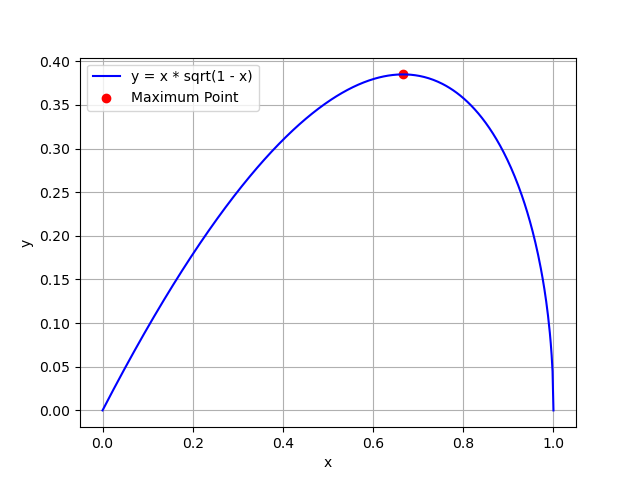
\includegraphics[width=0.75\columnwidth]{figs/fig22.png}
\end{center}

\end{document}